
\section{Resultados}

En esta sección se van a presentar los resultados obtenidos tras realizar el estudio del fenotipo Disgrafía.

\subsection{Red de genes asociados}

Después de descargar la red de genes asociados a la Disgrafía de la HPO, observamos que contenía 51 genes. Posteriormente, obtuvimos una red de genes relacionados con la Disgrafía utilizando la base de datos STRING-DB, la cual se puede observar en la imagen \ref{fig:genesAsociados}.

\begin{figure}[h!]
	\centering
	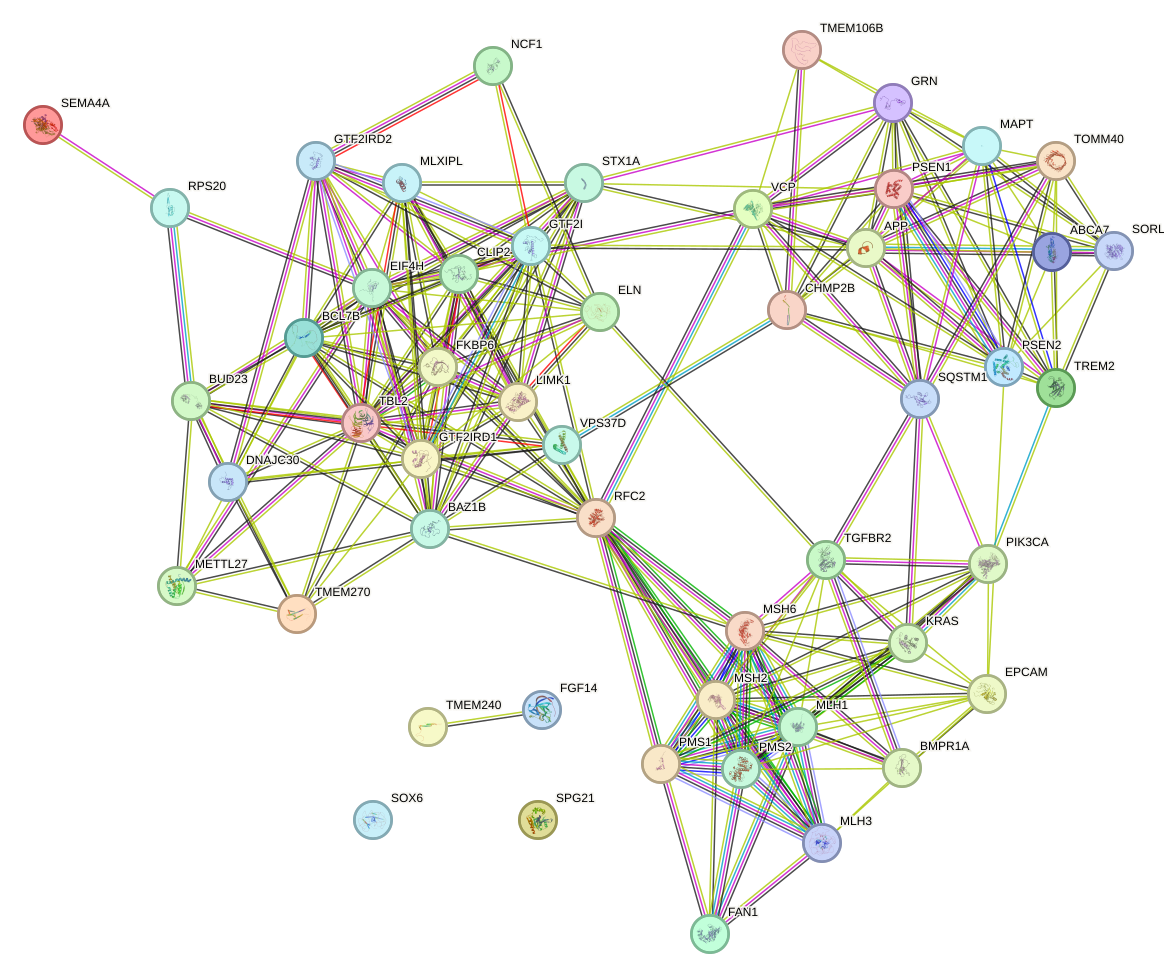
\includegraphics[width=0.7\textwidth]{figures/stringdb_51_genes.png}
	\caption{Red de genes asociados}
	\label{fig:genesAsociados}
\end{figure}

Se aplicó el algoritmo Diamond para propagar la red de genes y descubrir potenciales genes adicionales relacionados con la Disgrafía. El resultado de este proceso se encuentra en el archivo "propagated\_genes.txt", que contiene un listado con 200 genes. Utilizando estos genes, se creó una red mediante la librería de String. La cabecera del archivo que contiene la red se puede visualizar en la tabla \ref{tabla:resultDiamond} (se han omitido algunas columnas del archivo para mejor visualización).

\begin{table}[h]
	\centering
	\caption{Red de genes con los resultados de Diamond}
	\label{tabla:resultDiamond}
	\begin{tabular}{|c|c|c|c|c|c|}
		\hline
		stringId\_A & stringId\_B & preferredName\_A & preferredName\_B & score \\
		\hline
		9606.ENSP00000013807 & 9606.ENSP00000265433 & ERCC1 & NBN & 0.7 \\
		9606.ENSP00000013807 & 9606.ENSP00000347232 & ERCC1 & BLM & 0.701 \\
		9606.ENSP00000013807 & 9606.ENSP00000494957 & ERCC1 & UBE2T & 0.702 \\
		9606.ENSP00000013807 & 9606.ENSP00000229769 & ERCC1 & FANCE & 0.71 \\
		\hline
	\end{tabular}
\end{table}

Cada fila de esta red contiene información sobre la interacción de dos proteínas. Las cuatro primeras columnas incluyen los identificadores de los dos genes que están interactuando (tanto el StringId como el nombre). La cuarta columna (\textit{score}) es la puntuación combinada, la cual ya se mencionó en la sección \ref{section:redProteinas}.


\subsection{Detección de comunidades}

Se realizó un análisis de detección de comunidades en la red ampliada de genes. El algoritmo greedy\_modularity\_communities de NetworkX se empleó para identificar conjuntos de genes más densamente conectados entre sí. Los resultados de este análisis se presentan en la imagen \ref{fig:comunidades}.

\begin{figure}[h!]
	\centering
	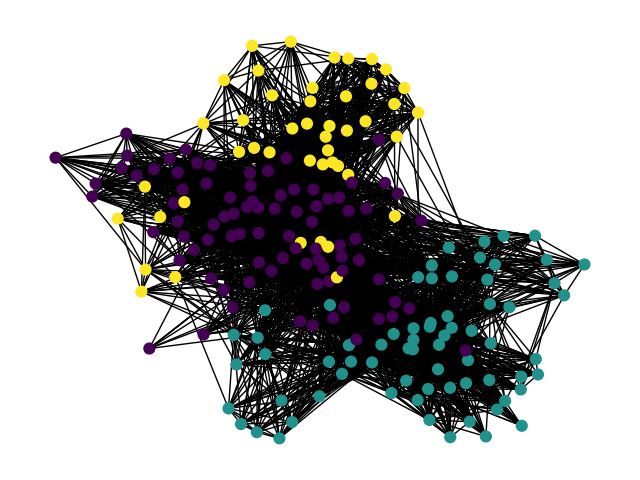
\includegraphics[width=0.7\textwidth]{../results/graph_communities.png}
	\caption{Comunidades de la red de genes}
	\label{fig:comunidades}
\end{figure}

Este algoritmo ha detectado tres comunidades. Cada color de la imagen \ref{fig:comunidades} representa una comunidad distinta.

\subsection{Enriquecimiento}

Se llevó a cabo un análisis de enriquecimiento funcional para identificar asociaciones significativas entre los genes y funciones específicas en procesos biológicos y rutas metabólicas. Este análisis se realizó tanto en el grafo ampliado como en cada una de las comunidades detectadas en la red de genes. La cabecera de los resultados se muestran en tablas \ref{tabla:enrique200}

Cada conjunto de resultados del enriquecimiento ha sido ordenado de manera ascendente según el false discovery rate (FDR).


\begin{table}[h]
	\centering
	\caption{Enriquecimiento grafo ampliado}
	\label{tabla:enrique200}
	\begin{tabular}{|c|c|c|c|c|}
		\hline
		category & number\_of\_genes & p\_value & fdr & description \\
		\hline
		Process & 181 & $4.35 \times 10^{-220}$ & $6.83 \times 10^{-216}$ & DNA metabolic process \\
		Process & 150 & $1.01 \times 10^{-184}$ & $7.94 \times 10^{-181}$ & DNA repair \\
		Process & 158 & $2.57 \times 10^{-176}$ & $1.34 \times 10^{-172}$ & Cellular response to DNA damage stimulus \\
		Process & 189 & $1.61 \times 10^{-160}$ & $6.32 \times 10^{-157}$ & Nucleic acid metabolic process \\
		RCTM & 122 & $2.07 \times 10^{-155}$ & $4.72 \times 10^{-152}$ & DNA Repair \\

		Keyword & 123 & $2.2 \times 10^{-147}$ & $1.48 \times 10^{-144}$ & DNA damage \\
		Process & 185 & $1.9 \times 10^{-142}$ & $4.96 \times 10^{-139}$ & Cellular macromolecule metabolic process \\
		\hline
	\end{tabular}
\end{table}